\documentclass[a4paper,11pt,fleqn]{scrartcl}%fleqn pour aligner les equations à gauche
\usepackage{../../Styles/Cours}


\newcommand{\chnum}{Chapitre 15}
\newcommand{\chtitle}{Les ondes mécaniques}
\newcommand{\dtype}{Cours}

\begin{document}
	\maketitle
    \section{Ondes mécaniques progressives}
     Une onde mécanique est une perturbation qui se propage dans un milieu matériel (contrairement aux ondes électromagnétiques qui peuvent se propager dans le vide).\\
    \textit{Exemple : }
        Le son, une onde le long d'une corde, une onde le long d'un ressort, des ondes sismiques, des vagues ...
    
    \subsection{Définition}
    \begin{minipage}{.58\linewidth}
    Une onde mécanique est \textbf{progressive} si la perturbation se propage dans le milieu matériel sans transport de matière. Il ne s'agit alors que d'un déplacement local et temporaire de particules.\\
    Une onde mécanique transporte avec elle de l'\textbf{énergie}.
\end{minipage}
    \begin{minipage}{.35\linewidth}
        \centering
        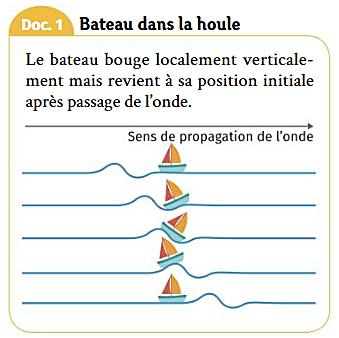
\includegraphics[width=\linewidth]{Ressources/1SPE_C15_Cours_Bateau.png}
    \end{minipage}

   
    \subsection{Grandeurs physiques associées aux ondes mécaniques}
    Pour étudier la propagation d'une onde mécanique, on mesure une grandeur physique qui varie, appelée \textbf{élongation}.\\
    \begin{minipage}{.45\linewidth}
        \textit{Exemple : }
    Pour la propagation d'une vague à la surface de l'eau, on mesure la hauteur de la vaque par rapport à la surface de l'eau au repos.
    \begin{center}
        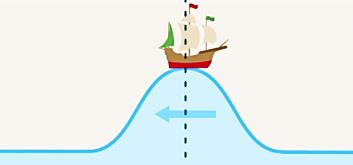
\includegraphics[width=\linewidth]{Ressources/1SPE_C15_Cours_Bateau2.png}
    \end{center}
    \end{minipage}\hspace{1em}
    \begin{minipage}{.5\linewidth}
        \small \centering
        \begin{tabular}{|>{\centering}m{.25\linewidth}|>{\centering}m{.225\linewidth}|>{\centering}m{.22\linewidth}|>{\centering \arraybackslash}m{.22\linewidth}|}
            \hline
            \textbf{Exemple d'onde mécanique} & Onde le long d'une corde & Onde le long d'un ressort & Onde onore dans l'air\\
            \hline
            \textbf{Milieu élastique de propagation} & Corde & Ressort & Air \\
            \hline
            \textbf{Élongation} & Distance d'un point de la corde par rapport à sa position de repos & Distance de la position d'une spire par rapport sa position de repos & Pression de l'air par rapport à la pression moyenne\\
            \hline
            
        \end{tabular}
    \end{minipage}
    

    \subsection{Ondes transversales et longitudinales}
    Lors du passage d'une onde, les particules du milieu sont momentanément mises en mouvement.\\
    \noindent \begin{minipage}{.53\linewidth}
        \begin{cours}
        Une onde est dite \textbf{transversale} si les particules du milieu vibrent perpendiculairement à la direction de propagation de l'onde.
    \end{cours}
    \begin{cours}
        Une onde est dite \textbf{longitudinale} si les particules du milieu vibrent dans la même direction que la direction de propagation de l'onde.
    \end{cours}
     Une onde mécanique longitudinale se propage par compressions et dilatations successives du milieu. C'est le cas des ondes sonores ou des ondes sismiques de type P.\\

    \end{minipage}\hspace{.02\linewidth}
    \begin{minipage}{.44\linewidth}
        \centering
        \includegraphics[width=\linewidth]{Ressources/Capture d’écran 2025-12-02 à 11.07.39.png}
    \end{minipage}
    

   
\section{La célérité d'une onde mécanique}
    \subsection{Le retard}
    Une onde progressive qui se propage atteint le point $M_1$ à un instant $t_1$ puis le point $M_2$ à un instant $t_2$.\\
    Le décalage temporel entre ces deux instants est appelé "retard" de l'onde.
    \begin{cours}
        Le \textbf{retard} d'une onde se propageant entre un point $M_1$ et un point $M_2$ est la durée séparant son passage entre ces deux points. il se note $\tau$ ("tau" dans l'alphabet grec) et se mesure en seconde. $$\tau = t_2 - t_1$$
    \end{cours}
    \begin{center}
        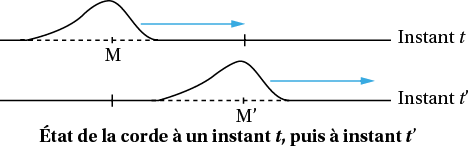
\includegraphics[width=.5\linewidth]{Ressources/retard.png}
    \end{center}

    \subsection{La célérité}
    Le terme "célérité" désigne la vitesse de propagation d'une onde progressive. On le différencie de la "vitesse" puisqu'il n'y a pas de propagation de la matière pour les ondes progressives. On la notera malgré tout "$v$".\\
    La célérité d'une onde dépend du type d'onde et également du milieu de propagation. plus le milieu est rigide, plus la célérité est grande.

    \newpage
    \begin{cours}
        Une onde se propageant d'un point $M_1$ à une point $M_2$ avec un retard $\tau$ a une célérité qui se calcule par :\\
        \begin{tabular}{>{\centering}m{.3\linewidth}|l}
        \multirow{3}{*}{$ v = \dfrac{M_1M_2}{\tau} = \dfrac{d}{\tau}$} & $M_1M_2$ ou $d$ la distance entre les points $M_1$ et $M_2$ en \unit{\meter}\\
        & $\tau$ le retard de l'onde entre les points $M_1$ et $M_2$ en \unit{\second}\\
        & $v$ la célérité de l'onde en \unit{\meter\per\second}\\
    \end{tabular}
    \end{cours}

    
    \begin{center}
        \begin{tabular}{|c|c|c|c|}
        \hline
        Milieu & Air & Eau & Acier\\
        \hline
        Célérité du son (\unit{\meter\per\second}) & 340 & 1500 & 5600\\
        \hline
    \end{tabular}
    \end{center}

    \begin{exemple}
        \begin{enumerate}
            \item Deux bouées, distantes de \SI{5,0}{km}, détectent une vague avec un retard de \SI{26}{\second}. Calculer la célérité de la vague.
            \item Calculer la distance parcourur par une onde en \SI{34}{min} si sa célérité est $v=\SI{2,7}{\meter\per\second}$.
            \item Une onde se déplace à la célérité $v=\SI{4,5}{\meter\per\second}$ dans un milieu. Calculer avec quel retard elle arrivera à un récepteur situé à \SI{240}{\centi\meter} de sa source.
        \end{enumerate}
    \end{exemple}
\newpage
\section{Les ondes mécaniques progressives périodiques}
Quand le phénomène à l'origine de l'onde mécanique progressive est périodique, chaque point du milieu de propagation subit une perturbation de manière préiodique. On peut donc dire que l'onde mécanique qui en résulte est \textbf{périodique}.
\begin{cours}
    Une onde mécanique progressive est \textbf{périodique} quand la perturbation se répère, identique à elle-même sur un intervalle de temps régulier. Un motif se pépète sur les courbes.
\end{cours}

    \subsection{La période et la fréquence}
    Si on prend un point à un "sommet" de l'onde périodique, celui-ci est soumis à une perturbation périodique (comme les autres points). Il descend puis remonte au cours du temps (pour une onde transversale). La période correspond à la durée nécessaire à ce point pour se retrouver à nouveau au sommet.
    \begin{cours}
        La \textbf{période} de l'onde est la plus petite durée nécessaire à un point du milieu pour retrouver la même position. Elle se note $T$ et se mesure en seconde.
    \end{cours}
    Elle se mesure avec la \textbf{durée d'un motif} sur une représentation temporelle de l'onde.
    \begin{cours}
        La \textbf{fréquence} de l'onde est le nombre de périodes par seconde. Elle se note $f$ et se mesure en hertz (\unit{\hertz}).
        \begin{center}
            \begin{tabular}{>{\centering}m{.3\linewidth}|l}
                \multirow{2}{*}{$ f = \dfrac{1}{T}$} & $f$ la fréquence en \unit{\hertz}\\
                & $T$ la période en \unit{\second}\\
            \end{tabular}
        \end{center}
    \end{cours}

    \subsection{La longueur d'onde}
    Deux points espacés d'une certaine distance qui suivent le même mouvement oscillent de la même phaçon. On dit qu'ils sont \textbf{en phase}. Ils sont dans le même "état vibratoire".
    \begin{cours}
        La \textbf{longueur d'onde} est la plus petite distance séparant deux points du milieu en phase. Elle se note $\lambda$ ("lambda" dans l'alphabet grec) et se mesure en mètre.
    \end{cours}
\end{document}